\section{Проектирование программного средства} % (fold)
\label{sec:development}

Разрабатываемым программное средство, как было отмечено в пункте~\ref{sub:domain:requirements:langs}, было разбито на три независимых модуля.
Каждый модуль разрабатывался отдельно. Модули обмениваются данными в определенном бинарном формате.
Это позволяет сторонним приложениям легко интегрироваться с разрабатываемым ПС путем реализации чтения описанных ниже бинарных форматов.

Диаграмма потоков данных изображена на рисунке~\ref{sec:development:data_flow_diagramm}.

\begin{figure}[ht]
  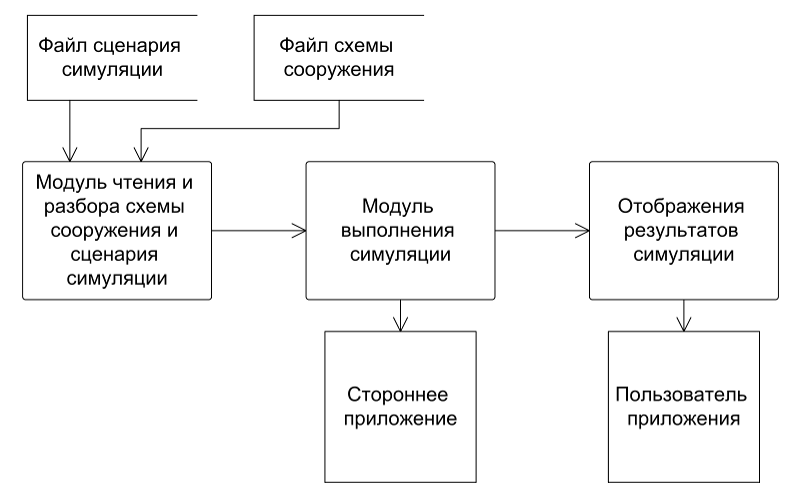
\includegraphics[width=\linewidth]{dfd}
  \caption{Диаграмма потоков данных}
  \label{sec:development:data_flow_diagramm}
\end{figure}

В данном разделе будут подробно рассмотрены все модули, используемые в разрабатываемом ПС, а также будут описаны бинарные форматы обмена данными.

\subsection{Модуль чтения и разбора схемы сооружения и сценария симуляции}
\label{sec:development:preprocessor}

Модуль чтения и разбора схемы сооружения и сценария симуляции выполнен на языке программирования Ruby~\cite{ruby_doc}.
В его задачи входит:
\begin{itemize}
  \item разбор сценария симуляции на отдельные компоненты;
  \item разбор схемы сооружения на отдельные компоненты;
  \item формирование сообщения о конфигурации модулю выполнения симуляции в определенном бинарном формате.
\end{itemize}

\subsubsection{Сценарий симуляции}
\label{sec:development:preprocessor:scenario_dsl}

Благодаря гибкости языка Ruby и его широких возможностей в метапрограммировании,
сценарий симуляции выполнен в виде предметно"=ориентированного языка (DSL "--- Domain Specific Language).

Пример сценария симуляции представлен на рисунке~\ref{sec:development:preprocessor:scenario_dsl_listing}.

\begin{figure}[ht!]
  \centering
  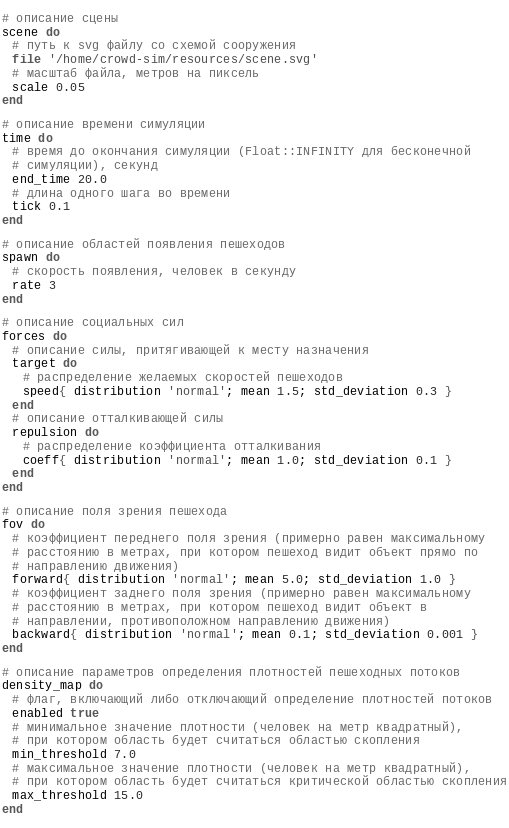
\includegraphics[width=\dimexpr\linewidth-8.5em\relax]{sim_params_example}
  \caption{Пример сценария симуляции}
  \label{sec:development:preprocessor:scenario_dsl_listing}
\end{figure}

В сценарии симуляции указывается множество различных параметров симуляции.
Более подробно данный язык и каждый его параметр будут рассмотрены в разделе~\ref{sec:manual:input:scenario}.
В данном разделе остановимся на рассмотрении вопросов, связанных с реализацией данного предметно"=ориентированного языка.

Основой разработанного модуля является класс Sections::Base. Он представляет собой базовый класс для определения секции в файле сценария симуляции.
Данный класс определяет статический метод field, который добавляет во внутренние переменные класса предоставленную информацию о поле сценария симуляции,
а также средствами метапрограммирования Ruby (в частности, с помощью метода define\_method) объявляет в вызывающем классе метод с именем, соответствующим имени поля.
Данный метод при вызове получает некоторое значение поля и сохраняет его во внутренней переменной объекта класса.
Таким образом, файл сценария симуляции по сути является файлом с Ruby кодом, который вызывает объявленные ранее методы с именами полей.

Поддерживаются следующие типы полей: целое число, число с плавающей точкой, строка, булевый флаг, потомок, распределение и динамический тип.

Потомок "--- особый тип поля, которому в параметрах передается имя класса, отвечающего за дальнейший разбор предоставленных параметров.
Данный тип поля использует такую особенность языка Ruby, как блоки, которые являются реализацией общей концепции замыканий.
В языке Ruby существует четыре концепции, описывающие некоторую совокупность кода "--- это block, Proc, lambda и method.

Proc "--- объект, описывает некоторую абстрактную совокупность кода. Он может быть сохранен в отдельную переменную. Доступ к коду, который хранит Proc, осуществляется с помощью метода call(args).
Lambda по своей сути практически не отличается от объекта Proc. Отличиями являются наличие контроля за передаваемыми аргументами и другое поведение оператора return внутри хранимого кода.
Method "--- объект-обертка над lambda. Используется для хранения методов внутри класса. Так же как Proc и lambda, использует метод call(args) для доступа к коду.

Блоки в руби являются своеобразным синтаксическим сахаром над описанными выше концепциями.
Они позволяют унифицировать доступ к определенным совокупностям кода с помощью единого синтаксиса.
В частности, любой метод в руби может принимать дополнительный последний параметр, отмеченный специальным символом \&.
В случае, если метод был вызван с блоком, в данный параметр передается сконвертированная в объект Proc совокупность кода, находящаяся в блоке.
Так же в Ruby присутствует функция yield, которая вызывает код, переданный в блоке, с определенными параметрами.

Таким образом, поле типа <<потомок>> принимает на вход блок, и выполняет его содержимое в контексте определенного класса-потомка.

Распределение "--- еще один особый тип поля. Он очень похож на <<потомка>>, за исключением того, что переданный блок всегда выполняется в контексте определенного класса (Utils::Distribution),
который отвечает за формирование определенных полей в зависимости от типа распределения (равномерное, нормальное и др.).

Последний тип поля "--- динамический тип. Он позволяет обрабатывающему классу определить некоторую совокупность кода, которая будет осуществлять разбор предоставленного значения.
В качестве совокупности кода может выступать любая из четырех описанных выше концепций.

\subsubsection{Схема сооружения}
\label{sec:development:preprocessor:svg_scheme}

В качестве схемы сооружения используется особым образом модифицированный SVG файл.
SVG~\cite{svg_home} "--- распространенный формат векторной графики на основе XML.
Выбор SVG в качестве формата для представления схемы сооружения обусловлен следующими причинами:
\begin{itemize}
  \item распространенность формата SVG;
  \item легкость модификации SVG элементов путем добавления атрибутов к соответствующим XML тегам;
  \item легкость разбора SVG файлов на компоненты.
\end{itemize}

Пример схемы сооружения представлен на рисунке~\ref{sec:development:preprocessor:svg_scheme_listing}.

\begin{figure}[!ht]
  \centering
  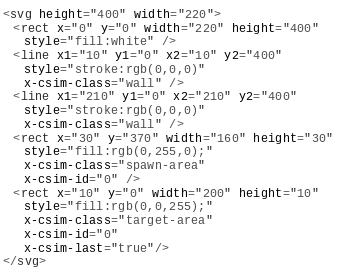
\includegraphics[width=\dimexpr\linewidth-4.2em\relax]{scene_example}
  \caption{Пример схемы сооружения}
  \label{sec:development:preprocessor:svg_scheme_listing}
\end{figure}

В реализованном ПС поддерживаются два основных элемента SVG "--- line и rect.
При этом введены следующие дополнительные атрибуты:
\begin{itemize}
  \item x-csim-class;
  \item x-csim-id;
  \item x-csim-seq-no;
  \item x-csim-last.
\end{itemize}

Атрибут x-csim-class отвечает за тип данного элемента.
Возможные значения:
  wall (препятствие),
  spawn\_area (место появления людей),
  target\_area (место назначения людей "--- промежуточное или конечное).

Атрибут x-csim-id отвечает за идентификацию определенного логического элемента.
В частности, он используется для связывания цепочки мест появления и мест назначения в единый путь.

Атрибут x-csim-seq-no может быть применен только к элементу с типом target\_area и определяет порядковый номер промежуточной target\_area.

Атрибут x-csim-last определяет, является ли данное место назначения промежуточным или конечным.

Поле, задающее путь к файлу со схемой сооружения в сценарии симуляции, имеет динамический тип.
В качестве обработчика указан метод класса Sections::Scene parse\_scene\_file.
Данный метод осуществляет разбор схемы сооружения с использованием библиотеки разбора XML Crack~\cite{ruby_crack_gem}, и сохраняет полученные геометрические элементы с их признаками.

\subsubsection{Формирование сообщения о конфигурации модулю выполнения симуляции}
\label{sec:development:preprocessor:format}

После разбора всех компонентов сценария симуляции модуль чтения и разбора должен сформировать сообщение о конфигурации модулю выполнения симуляции.
Для выполнения данной задачи каждый класс, представляющий собой секцию в файле конфигурации, обязан предоставить метод to\_config, который сформирует бинарную строку по определенному формату.
Данный метод вызывается рекурсивно для всех потомков, что позволяет на вершине дерева собрать все необходимое сообщение о конфигурации.

Формат описания конфигурации состоит из отдельных независимых друг от друга элементов.
Каждый элемент имеет следующую структуру:
\begin{itemize}
  \item идентификатор секции, к которой принадлежит данный элемент (1 байт);
  \item идентификатор элемента внутри данной секции (2 байта);
  \item данные элемента, закодированные в бинарном формате (переменное количество байт).
\end{itemize}

Подробно данные каждого элемента описаны в таблице~\ref{sec:development:preprocessor:format_table}.
Все координаты представлены двухбайтовыми целыми числами без знака, а перед каждой строкой записана ее длина.
Также используется формат распределения, который во всех случаях состоит из одного однобайтового целого без знака и двух чисел с плавающей точкой.
Первое число определяет тип распределения "--- равномерное (0x01) или нормальное (0x02).
В случае равномерного два числа с плавающей точкой означают границы <<от>> и <<до>> распределения,
а в случае нормального "--- среднее значение и среднеквадратичное отклонение соответственно.

\begin{longtable}[ht]{| >{\centering}m{0.25\textwidth}
                      | >{\centering}m{0.25\textwidth}
                      | >{\centering\arraybackslash}m{0.40\textwidth}|}
\caption{Формат сообщения о конфигурации} \label{sec:development:preprocessor:format_table}\tabularnewline

\hline Секция & Элемент & Данные элемента \tabularnewline
\endfirsthead
\captionsetup{labelformat=stbtablecont,justification=raggedright}
\caption[]{}\tabularnewline
\hline 1 & 2 & 3 \tabularnewline
\endhead
  \hline Сцена "--- 0x01 & Стена (препятствие) "--- 0x0001 & \specialcell{координаты первой точки\\
                                                                       (x0, y0)\\
                                                                       координаты второй точки\\
                                                                       (x1, y1)} \tabularnewline
  \hline Сцена "--- 0x01 & Место появления людей "--- 0x0002 & \specialcell{координаты первой точки\\
                                                                           (x0, y0)\\
                                                                           координаты второй точки\\
                                                                           (x1, y1)\\
                                                                           идентификатор пути (1 байт)} \tabularnewline
  \hline Сцена "--- 0x01 & Место назначения "--- 0x0003 & \specialcell{координаты первой точки\\
                                                                       (x0, y0)\\
                                                                       координаты второй точки\\
                                                                       (x1, y1)\\
                                                                       идентификатор пути\\
                                                                       (целое, 1 байт)\\
                                                                       порядковый номер\\
                                                                       (целое, 7 бит)\\
                                                                       флаг конечности (1 бит)} \tabularnewline
  \hline Сцена "--- 0x01 & Ширина, пикселей "--- 0x0011 & ширина (целое, 2 байта) \tabularnewline
  \hline Сцена "--- 0x01 & Высота, пикселей "--- 0x0012 & высота (целое, 2 байта) \tabularnewline
  \hline Сцена "--- 0x01 & Масштаб, метров на пиксель "--- 0x0013 & масштаб (с плавающей точкой, 8 байт) \tabularnewline
  \hline Сцена "--- 0x01 & Имя файла со сценой "--- 0x00FF & имя файла (строка) \tabularnewline

  \hline Параметры времени "--- 0x02 & Время окончания симуляции, секунд "--- 0x0001 & время (целое, 4 байта) \tabularnewline
  \hline Параметры времени "--- 0x02 & Единичный шаг времени, секунд "--- 0x0002 & шаг (с плавающей точкой, 8 байт) \tabularnewline

  \hline Параметры места появления "--- 0x03 & Скорость появления, человек в секунду "--- 0x0001 & скорость (с плавающей точкой, 8 байт) \tabularnewline

  \hline Параметры сил "--- 0x04 & Коэффициент отталкивания "--- 0x0101 & коэффициент (распределение) \tabularnewline
  \hline Параметры сил "--- 0x04 & Желаемая скорость передвижения "--- 0x0201 & скорость (распределение) \tabularnewline

  \hline Параметры поля зрения "--- 0x05 & Коэффициент переднего поля зрения "--- 0x0001 & коэффициент (распределение) \tabularnewline
  \hline Параметры поля зрения "--- 0x05 & Коэффициент заднего поля зрения "--- 0x0002 & коэффициент (распределение) \tabularnewline

  \hline Параметры определения плотности "--- 0x06 & Флаг включения "--- 0x0001 & \specialcell{флаг (1 байт)\\
                                                                                               1 "--- включено\\
                                                                                               0 "--- выключено} \tabularnewline
  \hline Параметры определения плотности "--- 0x06 & Минимальный порог плотности (ниже данного порога область не считается областью скопления) "--- 0x0002 & порог (с плавающей точкой, 8 байт) \tabularnewline
  \hline Параметры определения плотности "--- 0x06 & Максимальный порог плотности (выше данного порога области не различаются между собой по цвету) "--- 0x0003 & порог (с плавающей точкой, 8 байт) \tabularnewline

  \hline
\end{longtable}

\subsection{Модуль выполнения симуляции}
\label{sec:development:core}

Модуль выполнения симуляции разработан на языке программирования Rust~\cite{rust_doc}.
В его задачи входит:
\begin{itemize}
  \item разбор и сохранение входного сообщения о конфигурации;
  \item выполнение симуляции по заданной конфигурации;
  \item в процессе выполнения непрерывно выдавать данные о текущем состоянии симуляции модулю отображения результатов.
\end{itemize}

\subsubsection{Разбор и сохранение конфигурации}
\label{sec:development:core:configuration}

Разбор и сохранение конфигурации осуществляется подмодулем con\-fi\-gu\-ra\-ti\-on.
Экспортируемыми элементами из данного модуля являются
функция new, которая осуществляет разбор предоставленной конфигурации и сохранение ее в новое хранилище,
макрос config, который получает значение определенного параметра из хранилища,
а также множество типов (структур и перечислений), используемых в качестве ключей для доступа к конфигурации.

В качестве хранилища для конфигурации была выбрана библиотека AnyMap~\cite{rust_anymap_cargo}.
Данная библиотека позволяет хранить по ключу в виде типа некоторое значение данного типа.
Соответственно, в модуле configuration объявлено по одному типу на каждый элемент конфигурации.

Основной цикл разбора конфигурации находится в функции par\-se\_con\-fig\_fi\-le.
Данная функция вызывает функцию par\-se\_sin\-gle\_item до тех пор, пока не останется ни одного необработанного элемента.

Функция parse\_single\_item читает из входного потока номер секции, и в зависимости от него вызывает одну из функций
par\-se\_sce\-ne\_item (секция сцены), par\-se\_time\_item (секция параметров времени),
par\-se\_spawn\_item (секция параметров мест появления),
par\-se\_for\-ces\_item (секция параметров социальных сил),
par\-se\_fov\_item (секция параметров поля зрения)
или par\-se\_den\-si\-ty\_map\_item (секция параметров плотностей потоков).
Каждая из этих функций читает из входного потока номер элемента конфигурации,
а потом в зависимости от элемента читает нужное количество параметров с помощью функций чтения элементарных типов.

В качестве функций чтения элементарных типов в модуле configuration реализованы:
par\-se\_u8 (чтение однобайтового беззнакового целого числа),
par\-se\_u16 (чтение двухбайтового беззнакового целого числа),
par\-se\_u32 (чтение четырехбайтового беззнакового целого числа),
par\-se\_f64 (чтение восьмибайтового числа с плавающей точкой),
par\-se\_string (чтение строки),
par\-se\_co\-or\-di\-na\-tes (чтение набора из четырех координат),
par\-se\_dis\-tri\-bu\-ti\-on (чтение элемента распределения).

\subsubsection{Выполнение симуляции}
\label{sec:development:core:simulation}

Выполнение симуляции осуществляется модулем si\-mu\-la\-ti\-on.
Вначале происходит инициализация процесса, при которой все подмодули симуляции получают нужные значения из конфигурации.

В модуле simulation объявлено два основных метода "--- main\_loop и update\_state.

Метод main\_loop в цикле выполняет следующие действия:
\begin{itemize}
  \item обновить состояние (update\_state);
  \item сформировать сообщений о текущем состоянии;
  \item передвинуть время симуляции на следующий шаг;
  \item повторять пока не достигнуто время конца симуляции.
\end{itemize}

Метод update\_state служит для обновления состояния симуляции и выполняет следующие действия:
\begin{itemize}
  \item рассчитывает итоговую силу для каждого пешехода;
  \item сдвигает каждого пешехода в соответствии с рассчитанной итоговой силой;
  \item создает новых пешеходов в областях появления;
  \item обрабатывает пешеходов, достигших своей точки назначения.
\end{itemize}

Для выполнения своих целей модуль симуляции использует следующие подмодули:
\begin{itemize}
  \item person;
  \item time;
  \item forces;
  \item scene.
\end{itemize}

Подмодуль person отвечает за представление одного пешехода.
Для каждого пешехода хранится следующая информация:
\begin{itemize}
  \item координаты пешехода;
  \item направление пешехода;
  \item идентификатор пути в сцене, по которому движется пешеход;
  \item текущая цель пешехода;
  \item структура, которая хранит параметры сил, характерные для данного пешехода (желаемая скорость, коэффициент отталкивания).
\end{itemize}

Основным методом, объявленным на классе Person, является метод перемещения под воздействием силы (move\_by).
Данный метод принимает результирующую силу, воздействующую на пешехода, и время.
Пешеход сдвигается на соответствующее расстояние, и новым направлением для него становится направление силы.

Также у класса Person есть вспомогательный метод reached\_destination, который определяет, достиг ли пешеход своей текущей цели.

Подмодуль time отвечает за управление временем симуляции и хранит текущее время, время окончания и время одного шага.
В нем объявлены следующие методы:
\begin{itemize}
  \item is\_passed "--- возвращает истину в случае, если достигнуто время окончания (симуляция закончена);
  \item next\_tick "--- переводит время симуляции на один шаг вперед.
\end{itemize}

Подмодуль forces отвечает за используемые при симуляции силы.
Он экспортирует два основных метода "--- расчет результирующей социальной силы (total\_force\_for\_person)
и метод генерации структуры параметров сил для нового пешехода (generate\_person\_forces\_param).

Метод расчета результирующей социальной силы использует аналог интерфейса (в языке Rust они называются traits) для получения значения каждой используемой социальной силы.
В данном интерфейсе определено, что сила получает на вход пешехода и сцену, и должна вернуть некоторый вектор воздействия на пешехода, а также точку источника силы.
Также стоит отметить, что для хранения всех используемых социальных сил используется единое перечисление.

После определения всех социальных сил, воздействующих на пешехода, осуществляется коррекция по полю зрения.
Для этого вектор каждой силы домножается на коэффициент, зависящий от формы поля зрения пешехода и направления к источнику силы.

После суммирования всех скорректированных социальных сил, воздействующих на пешехода, проверяется, повернут ли пешеход в нужную сторону (в сторону результирующей силы).
Если же пешеход не повернут в нужную сторону, то происходит перерасчет новой силы поворота (которая не так сильно отличается от исходного направления пешехода) с ограниченным модулем.
Таким образом, пешеход не может мгновенно развернуться, что добавляет модели реалистичности.

Последним подмодулем является scene.
Он является контейнером для всех объектов моделирования (пешеходов, препятствий, путей следования).
Для большинства объектов моделирования в качестве примитива хранения выбран вектор (абстракция над массивом динамической длины в куче).
Это обусловлено тем, что большинство объектов на сцене статичны и не меняются.
Однако данное утверждение не справедливо для пешеходов, в связи с чем для их хранения используется другой примитив "---
двусвязный список с использованием его реализации LinkedList~\cite{rust_linked_list_cargo}. Это позволяет быстро удалять пешеходов из середины списка.

Важными экспортируемыми методами модуля scene являются spa\-wn\_peo\-ple, pro\-cess\_reach\-ed\_des\-ti\-na\-ti\-on\_people, и get\_den\-si\-ty\_map.

Метод spawn\_people отвечает за создание новых пешеходов в областях появления пешеходов.
Сначала метод выбирает свободное место для пешехода внутри области появления.
Для этого он некоторое конечное число раз пытается случайно сгенерировать координаты внутри данной области.
Если все сгенерированные координаты были заняты, то в системный лог пишется предупреждение о том, что область появления переполнена.
Если же место для пешехода нашлось, то создается новый объект класса Person.

Метод process\_reached\_destination\_people отвечает за следование пешеходами вдоль их пути.
Данный метод выбирает тех пешеходов, которые достигли своей текущей цели.
Далее производится проверка, была ли достигнутая пешеходом цель, которая является последней в цепочке.
Если да, то данный пешеход удаляется как достигший своей цели. Если нет, то в качестве текущей цели пешеходу проставляется следующая по цепочке цель.

Метод get\_density\_map отвечает за расчет карты плотностей пешеходных потоков.
Он использует следующий алгоритм определения плотности в каждой точке сцены:
\begin{itemize}
  \item инициализировать двумерный массив плотностей нулями;
  \item для каждого пешехода внутри сцены:
  \item для каждой точки на некотором расстоянии от пешехода:
  \item добавить в данную точку значение плотности, зависящее от расстояния до пешехода.
\end{itemize}

В качестве зависимости плотности от расстояния до пешехода выбрана аппроксимация гауссового распределения.
Таким образом, мы получаем непрерывную плавную карту плотностей пешеходных потоков внутри сцены.

\subsubsection{Вспомогательные подмодули, используемые при симуляции}
\label{sec:development:core:utils}

При выполнении симуляции использовались некоторые вспомогательные подмодули в составе модуля utils.

Первым таким подмодулем является подмодуль linelg "--- реализация линейной алгебры~\cite{linelg_book}.
В нем реализованы структуры данных и операции над такими сущностями, как точка, вектор, линия, расстояние и др.
При разработке данного модуля широко использовались возможности языка Rust по перегрузке операторов,
что позволило сделать код, использующий данный модуль, более лаконичным.

Вторым подмодулем является distributions "--- реализация генерирования значения случайной величины, описанной определенной структурой.
Генерирование значения для равномерного распределения осуществляется методом обратной функции,
а для нормального распределения "--- методом на основе центральной предельной теоремы~\cite{probability_modeling}.

\subsubsection{Формирование сообщений о текущем состоянии симуляции модулю отображения результатов}
\label{sec:development:core:output}

За формирование сообщений о текущем состоянии симуляции отвечает подмодуль output.
Так же как и модуль simulation, при инициализации он принимает объект конфигурации, из которого он получает нужные ему элементы.

Формат сообщений модулю отображения результатов можно разбить на два отдельных сообщения: инициализирующее сообщение и сообщение о текущем состоянии.

Посылку инициализирующего сообщения осуществляет метод se\-nd\_in\-it.
В составе инициализирующего сообщения посылается информация в следующем порядке:
\begin{itemize}
  \item длина строки с именем svg файла схемы сооружения (беззнаковое число, 2 байта);
  \item строка с именем svg файла схемы сооружения;
  \item масштаб svg файла схемы сооружения, метров на пиксель (число с плавающей точкой, 8 байт);
  \item флаг наличия карт плотности пешеходных потоков: 1 "--- есть, 0 "--- нету (беззнаковое число, 1 байт);
  \item минимальная плотность пешеходных потоков (число с плавающей точкой, 8 байт);
  \item максимальная плотность пешеходных потоков (число с плавающей точкой, 8 байт).
\end{itemize}

После этого на каждом такте осуществляется посылка сообщения о текущем состоянии с помощью метода dump\_state.
Каждое сообщение о текущем состоянии состоит из следующих полей:
\begin{itemize}
  \item текущее время симуляции (число с плавающей точкой, 8 байт);
  \item в случае, если карты плотности пешеходных потоков включены: флаг наличия в данном сообщении информации о плотности пешеходных потоков (беззнаковое число, 1 байт);
  \item в случае, если флаг наличия информации о плотности пешеходных потоков установлен: количество точек с плотностью выше минимальной (беззнаковое число, 4 байта);
  \item в случае, если флаг наличия информации о плотности пешеходных потоков установлен: массив из точек с повышенной плотностью в формате
    координата по горизонтали (беззнаковое число, 2 байта), координата по вертикали (беззнаковое число, 2 байта), плотность (число с плавающей точкой, 8 байт);
  \item количество пешеходов (беззнаковое число, 4 байта);
  \item массив из координат пешеходов и их направлений в формате
    координата по горизонтали (беззнаковое число, 2 байта), координата по вертикали (беззнаковое число, 2 байта), направление (число с плавающей точкой, 8 байт).
\end{itemize}

Важным моментом является опциональное присутствие карты плотности в сообщении.
Это обусловлено тем, что расчет карты плотности достаточно трудоемкая задача, и делать данный расчет на каждой итерации симуляции не имеет смысла.
Вместо этого, расчет карты плотности производится каждую секунду модельного времени.

Также стоит упомянуть, что направление представляет собой угол от положительного направления оси абсцисс в радианах и имеет область значений от $0$ до $2\pi$.

\subsection{Модуль отображения результатов симуляции}
\label{sec:development:animator}

Модуль отображения результатов симуляции выполнен на языке программирования С с использованием библиотеки SDL~\cite{libsdl_home}.
В его задачи входит:
\begin{itemize}
  \item реализация ожидания следующего состояния в случае, если модуль выполнения симуляции не успевает слать данные в режиме реального времени;
  \item разбор данных о текущем состоянии симуляции;
  \item отображение текущего состояния симуляции на экране.
\end{itemize}

\subsubsection{Реализация ожидания следующего состояния симуляции}
\label{sec:development:animator:wait}

В качестве реализации ожидания следующего состояния был выбран системный вызов select,
который позволяет заблокировать текущий поток на определенное время (или на неограниченное время),
до тех пор пока переданные ему файловые дескрипторы не станут доступны для чтения, записи либо чтения ошибки.

Таким образом, перед началом каждого цикла считывания текущего состояния реализуемый модуль вызывает функцию select с дескриптором на чтение и засыпает до тех пор,
пока от модуля выполнения симуляции не придут данные.

\subsubsection{Разбор данных о текущем состоянии симуляции}
\label{sec:development:animator:parse}

По причине простоты формата сообщения о текущем состоянии симуляции, операции по их разбору не вынесены в отдельный подмодуль и осуществляются прямо в главном цикле данного модуля.
Для осуществления чтения элементарных типов в контроллере объявлены следующие методы:
\begin{itemize}
  \item unsigned char controller\_read\_byte();
  \item unsigned short controller\_read\_short();
  \item unsigned long controller\_read\_long();
  \item char* controller\_read\_string();
  \item double controller\_read\_double().
\end{itemize}

\subsubsection{Отображение текущего состояния симуляции на экране}
\label{sec:development:animator:show}

Последовательность действий модуля отображения текущего состояния симуляции следующая:
\begin{itemize}
  \item проинициализировать все системы библиотеки SDL;
  \item прочитать инициализационное сообщение от модуля выполнения симуляции;
  \item загрузить и подготовить все необходимые текстуры из SVG файлов;
  \item войти в главный цикл;
  \item осуществить очистку всех используемых ресурсов.
\end{itemize}

При этом в главном цикле выполняются следующие задачи:
\begin{itemize}
  \item ожидать сообщения о следующем состоянии симуляции от модуля выполнения симуляции;
  \item прочитать время симуляции пакета данных;
  \item очистить экран;
  \item вывести на экран текстуру со сценой;
  \item если присутствует информация о плотностях: прочитать данную информацию, сформировать и отобразить текстуру с плотностями;
  \item прочитать и отобразить информацию о пешеходах;
  \item рассчитать текущее время симуляции как разницу между текущим временем и временем начала симуляции;
  \item если текущее время симуляции меньше чем время пакета данных, ожидать нужное количество времени;
  \item обновить экран новыми данными.
\end{itemize}

Загрузка и растеризация SVG файлов осуществлялась с помощью библиотек librsvg~\cite{librsvg_home} и cairo~\cite{cairo_home}.

Все описанные выше задачи достаточно просты, некоторых пояснений требуют лишь формирование текстуры с плотностями пешеходных потоков и отображение информации о пешеходах.

Формирование текстуры с плотностями пешеходных потоков осуществляется следующим образом:
сначала структура хранения информации о цвете областей очищается,
а затем для каждого пикселя с информацией о плотности вычисляется его цвет.
Цвет для пикселя с информацией о плотности определяется по следующим правилам:
некоторое константное значение в канале прозрачности,
константное максимальное значение в канале красного цвета и
значение, которое определяется как разница между максимальным значением цвета и масштабированным значением плотности от 0 до максимального значения цвета
в соответствии с параметрами минимального и максимального порогов плотностей в каналах синего и зеленого цвета.
Таким образом, цвет области меняется от ярко-красного для плотностей равных или выше максимального порога до белого для плотностей равных либо меньших минимального порога.

При отображении информации о пешеходах возникла проблема поворота текстур пешехода на некоторый угол.
При загрузке и подготовке текстур из SVG файла осуществляется масштабирование текстур до нужного размера и растеризация.
Однако поворот растеризованных текстур низкого разрешения вокруг своей оси приводил к появлению значительных артефактов.
Для решения данной проблемы был реализован следующий подход: поворот на некоторый набор дискретных углов осуществляется в векторном виде при загрузке SVG файлов.
Таким образом, мы получаем некоторый дискретный набор (в реализованном ПС использовалась дискретизация по 1 градусу) уже повернутых текстур более высокого качества.
При отображении конкретного пешехода мы просто выбираем текстуру, повернутую на нужный угол.
